% Drawing 85/05-7 -- folder 85, batch 05, archive page 93 (PDF page 94).
% Transcription: en dessous à gauche, un tétraèdre : sommets $s$ (en haut) et $s'$ (à droite), l'arête du premier plan descendant de $s$, une arête marquée $a$ (à gauche) et une face marquée $f$, l'arête cachée en pointillé
% Kind: tetrahedron with labels s, s', a, f. Method 2 (schematic redraw from the facsimile). Status: ok.
% Notes: Ink. Four vertices, five visible edges, the hidden edge from the left vertex to s' dashed (its first stretch solid, as on the page); a beside the left edge from s, f in the left face, three light pencil strokes of hatching in that face. Redrawn 2026-11-12 (issue 128): to check again.
% Coordinates: 1 unit = 1 mm = 1/100 of the crop width (bbox in page fractions: [0.12, 0.11, 0.32, 0.24]).
% Redrawn by Claude (claude-fable-5-2), issue #128, 2026-11-12; not checked by a human; not compiled (no TeX in the session).
% Rights: reproduces part of the work -- behind RENDER_TRANSCRIPTS, never published by itself.
\documentclass[tikz,border=3pt]{standalone}
\usepackage{amsmath,amssymb}
\usetikzlibrary{patterns,arrows.meta}
\tikzset{pencil/.style={black!45}, struck/.style={black!35}, mpt/.style={circle,draw,inner sep=1.3pt}, pt/.style={circle,fill,inner sep=0.9pt}, opt/.style={circle,draw,fill=white,inner sep=1.1pt}}
\begin{document}
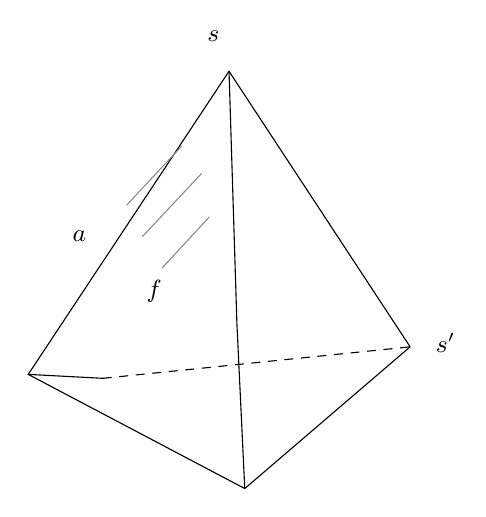
\begin{tikzpicture}[x=1mm,y=1mm,line cap=round,line join=round,font=\scriptsize]
\draw (49,-28) -- (23.5,-66.5) -- (51,-81) -- (72,-63) -- (49,-28);
\draw (49,-28) -- (50,-60) -- (51,-81);
\draw (23.5,-66.5) -- (33,-67);
\draw[dashed] (33,-67) -- (72,-63);
\draw[pencil] (36,-45) -- (43,-37.5);
\draw[pencil] (38,-49) -- (45.5,-41);
\draw[pencil] (40.5,-53) -- (46.5,-46.5);
\node[inner sep=1pt] at (47,-23.5) {\small $s$};
\node[inner sep=1pt] at (76.5,-62.5) {\small $s'$};
\node[inner sep=1pt] at (30,-49) {\small $a$};
\node[inner sep=1pt] at (39.5,-56) {\small $f$};
\end{tikzpicture}
\end{document}
